\documentclass{beamer}
\usetheme{metropolis}
\usepackage{listings}
\usepackage{graphicx}
\usepackage{standalone}
\usepackage{tikz}
\usepackage{tabu}
\usepackage{tikz}
\usepackage{verbatim}
\usepackage{tcolorbox}
\usepackage{appendixnumberbeamer}
\usepackage{booktabs}
\usepackage[scale=2]{ccicons}
\usepackage{pgfplots}
\usepackage{xspace}
\usepgfplotslibrary{dateplot}
\usetikzlibrary{shapes,snakes}

\setbeamertemplate{frame footer}{\insertsection\ // \insertsubsection}

\title{User, Group and Rights Management for Cloud Providers}
\subtitle{Fachpraktikum Information Systems}
\author{Christoph Kleine, Tim Zwietasch, Constantin Weißer}
\date{\today}

\begin{document}

\frame{\titlepage}

\section{Introduction}
\subsection{Idea}
\begin{frame}
	\frametitle{Motivation}
	\begin{tcolorbox}[title=Overall Goal]
		Create an ECM portal for companies that do not want to host
		their data with one of the big providers. The focus is on
		usability and user-friendliness while maintaining security.
	\end{tcolorbox}

	\begin{itemize}
		\item Many companies prefer domestic small solutions
		\item Keep advantages of cloud solutions
		\item IBM's commercial portal as a model
	\end{itemize}
\end{frame}

\begin{frame}
	\frametitle{Motivation}
	\begin{tcolorbox}[title=Our Goal]
		Develop the user, groups and role management for this ECM portal
		based on open-source software.
	\end{tcolorbox}
	\begin{itemize}
		\item Easily extendible web application
		\item Usability
		\item Free and Open-Source Software (FOSS)
	\end{itemize}
\end{frame}

\begin{frame}
	\frametitle{Open Source Software}
	\begin{tcolorbox}[title=Why use FOSS components?]
		\begin{itemize}
			\item no licensing costs
			\item scalability!
			\item high security standards
			\item adaptivity
		\end{itemize}
	\end{tcolorbox}
\end{frame}

\section{Architecture}
\subsection{Overview}
\begin{frame}
	\frametitle{Architecture}
	\begin{columns}[T]
		\begin{column}{0.48\textwidth}
			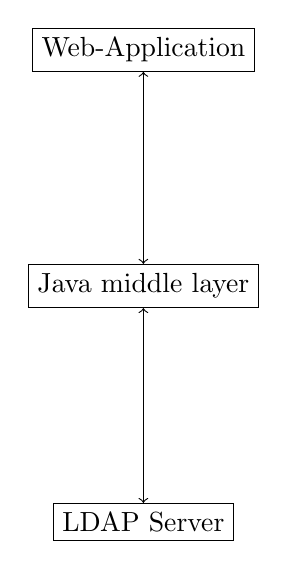
\begin{tikzpicture}
				\tikzset{every rectangle node/.style={draw, rectangle}}
				\node (frontend) at (0, 3) {Web-Application};
				\node (middleend) at (0, 0) {Java middle layer};
				\node (ldap) at (0, -3) {LDAP Server};

				\draw[<->] (frontend) to[] (middleend);
				\draw[<->] (middleend) to[] (ldap);
			\end{tikzpicture}
		\end{column}
		\begin{column}{0.48\textwidth}
			\begin{itemize}
				\item Web-Application as user interface
				\item Java middle layer as intermediate program logic
				\begin{itemize}
					\item provides REST interface
					\item accepts action requests
					\item provides response
				\end{itemize}
			\item LDAP-Server as persistent storage
			\end{itemize}
		\end{column}
	\end{columns}
\end{frame}

\section{Questions?}

\end{document}
